\documentclass[../manuale-sviluppatore.tex]{subfiles}

\begin{document}

\subsection{Server}%
\label{sub:server}

\subsubsection{Installazione Docker}%
\label{subs:installazione_docker}

La prima cosa che l'utente deve fare è verificare l'edizione dell'attuale versione di Windows 10. Aprire la barra di ricerca ed eseguire il comando \textit{winver}.

\begin{figure}[H]
  \centering
  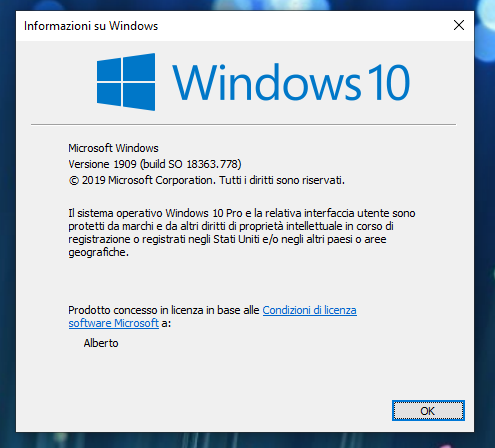
\includegraphics[width=90mm]{winver.png}
  \caption{Risultato winver}%
  \label{fig:risultato_winver}
\end{figure}

Una volta individuata l'edizione, installare:
\begin{description}
  \item[Docker Desktop] se l'edizione di Windows 10 è Professional oppure Enterprise.
  \item[Docker Toolbox] altrimenti.
\end{description}

Nel caso di \textbf{Docker Desktop}, eseguire queste operazioni:
\begin{itemize}
  \item installare l'applicazione Docker Desktop, al seguente \href{https://hub.docker.com/editions/community/docker-ce-desktop-windows}{indirizzo}.
  \item aprire la barra di ricerca, digitare \textit{Docker Desktop} ed eseguire l'applicazione.
  \item attendere qualche secondo per l'esecuzione di Docker Desktop, poi andare sulla barra delle applicazioni in \textit{Mostra icone risposte} e accertarsi che l'icona dell'applicazione (una balena bianca) sia presente e che, facendo un hover sopra l'icona appaia il messaggio \textit{Docker is running}.
  \item cliccare con il tasto destro sull'icona per aprire il menu, e cliccare sulla voce \textit{Switch to Linux containers} per attivare il daemon Linux con cui la
  Docker \glossarioLocale{CLI} interagisce e quindi utilizzare i contenitori Linux.
\end{itemize}
\newpage

Nel caso di \textbf{Docker Toolbox}, seguire i passi per l'installazione dell'applicazione che si trovano al seguente \href{https://docs.docker.com/toolbox/toolbox_install_windows/}{indirizzo}.
Va precisato che Docker Toolbox lavora dentro una \glossarioLocale{VM}; in questo modo i container non vengono eseguiti sull'indirizzo localhost ma sull'\glossarioLocale{IP} della VM\@.
Per risolvere questo problema, eseguire queste operazioni per la configurazione del \glossarioLocale{port forwarding}:
\begin{itemize}
  \item selezionare la VM su cui parte Docker (segnato in rosso).
  \item selezionare la voce \textit{Settings} della VM (segnato in arancione scuro).
  \item selezionare la tab \textit{Network} (segnato in arancione chiaro).
  \item cliccare sul pulsante \textit{Port Forwarding} (segnato in arancione scuro).

  \begin{figure}[H]
    \centering
    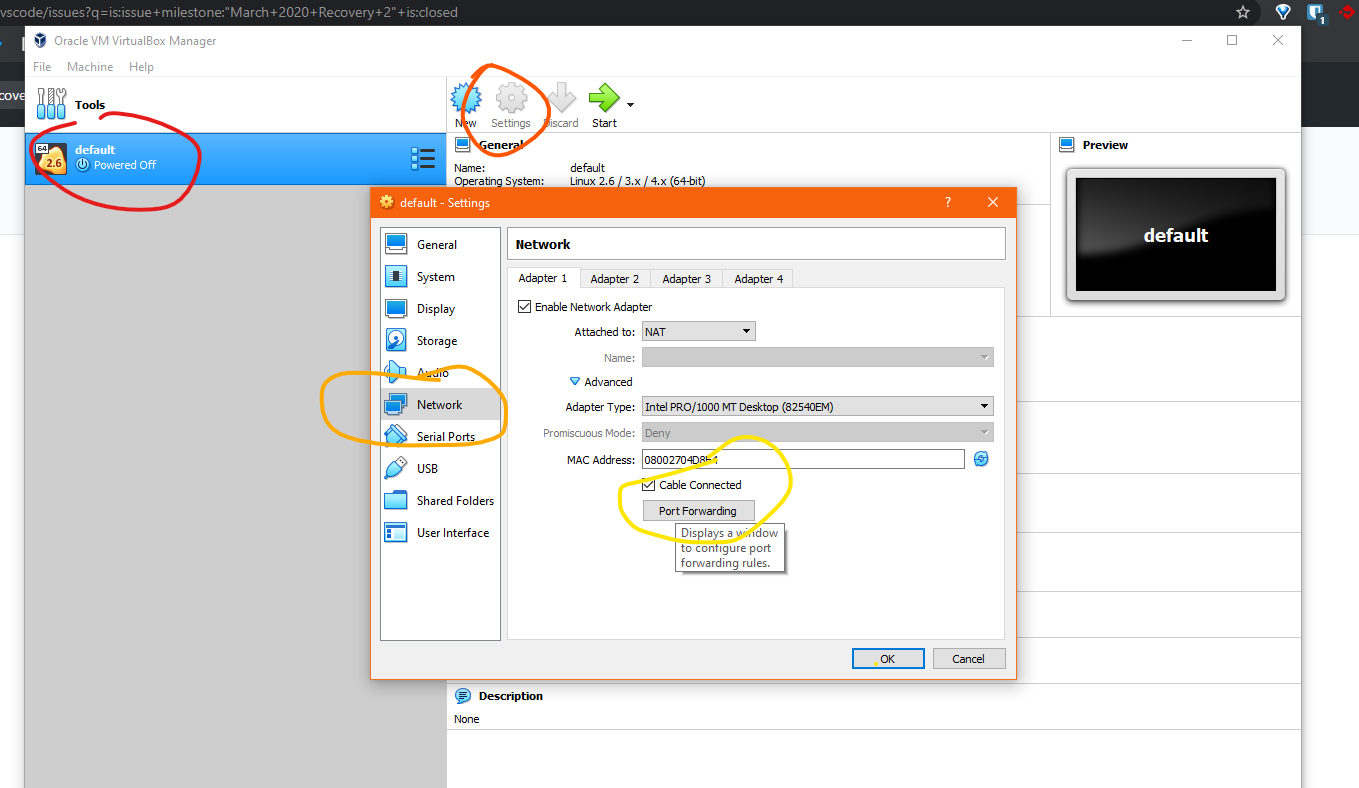
\includegraphics[width=110mm]{virtualbox-port-forwarding-1.png}
    \caption{Port forwarding-Parte 1}%
    \label{fig:port_forwarding_parte_1}
  \end{figure}

  \item aggiungere, se necessario, il nome del servizio con la quale Docker deve comunicare, con annesso tipo di protocollo e le porte, rispettivamente quella pubblicata da VirtualBox (segnata in rosso), e quella pubblicata dal container alla VM (segnata in giallo). Non è necessario che le due porte siano uguali: per dettagli, visitare il seguente \href{https://docs.docker.com/config/containers/container-networking/#published-ports#published-ports}{indirizzo}.

  \begin{figure}[H]
    \centering
    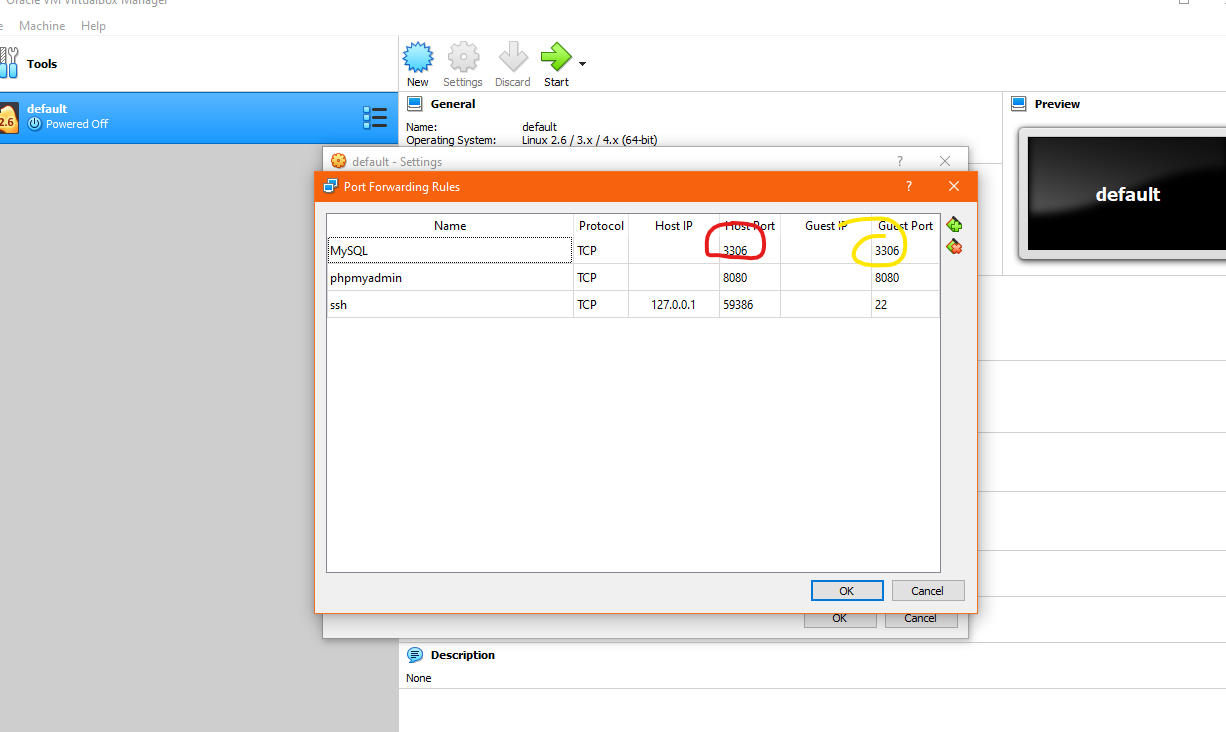
\includegraphics[width=110mm]{virtualbox-port-forwarding-2.png}
    \caption{Port forwarding-Parte 2}%
    \label{fig:port_forwarding_parte_2}
  \end{figure}
\end{itemize}
\newpage

\subsubsection{Avvio dei servizi}%
\label{subs:avvio_dei_servizi}

Per la gestione delle dipendenze, utilizziamo Gradle.

All'interno della repository \textit{Gruppone/stalker-server}, è presente una coppia di script (\textit{gradlew} per linux e \textit{gradlew.bat} per Windows) che permette di eseguire i task necessari senza bisogno di installare \glossarioLocale{Gradle}.

Il comando da utilizzare per eseguire il server e renderlo raggiungibile all'indirizzo \href{localhost:11111}{localhost:11111} è: \par\bigskip

\begin{center}
  \textit{./gradlew bootRun}
\end{center}
\par\bigskip

Spring utilizza una funzione chiamata \glossarioLocale{LiveReload}: consente una compilazione automatica ad ogni modifica del codice sorgente in modo da non riavviare manualmente l'esecuzione del server Spring e velocizzare il lavoro.

Una volta avviato il server, lo strato di persistenza, che è rappresentato dal database MySQL, non è ancora attivo.

Il comando per avviarlo deve essere eseguito dalla root nel server, ed è il seguente: \par\bigskip

\begin{center}
  \textit{docker-compose up -d rdb}
\end{center}
\par\bigskip

\textbf{rdb} (\glossarioLocale{Relational Database}) è il nome del servizio definito all'interno di quei file.

Per conoscere tutti i dettagli dei container che possono essere istanziati, cercare dalla root del server i file \emph{docker-compose.yml} e \emph{docker-compose.override.yml}.

E' anche possibile far partire più di un servizio alla volta con: \par\bigskip

\begin{center}
  \textit{docker-compose up -d rdb rdb-gui}
\end{center}

\par\bigskip

Questo comando fa partire un'istanza di MySQL e allo stesso tempo un'istanza di PhpMyAdmin, con la quale è possibile interagire con il database attraverso un'interfaccia grafica web all'indirizzo \href{localhost:8080}{localhost:8080}.

Esiste un comando generale che fa partire tutti i servizi disponibili, ovvero: \par\bigskip

\begin{center}
  \textit{docker-compose up -d}
\end{center}
\par\bigskip

\textbf{-d}  sta per --detached, ovvero serve a ritornare il prompt dopo che Docker ha avviato il \glossarioLocale{container}.

L'utente può provare ad eseguire gli stessi comandi senza il -d per notare la differenza.

Il teardown completo dei servizi che compongono lo strato di persistenza (ovvero lo spegnimento di tutti i container, e quindi di tutti i servizi) si esegue con il comando: \par\bigskip

\begin{center}
  \textit{docker-compose down --rmi all --remove-orphans --volumes}
\end{center}
\par\bigskip

Si consiglia l'utente di eseguire questo comando con frequenza, in modo da evitare che il funzionamento del server dipenda da azioni svolte su una specifica istanza del database.

\end{document}
